\documentclass[conference]{IEEEtran}
\usepackage{amsmath,amssymb,amsfonts}
\usepackage{graphicx}
\usepackage{algorithm}
\usepackage{algorithmic}
\usepackage{booktabs}
\usepackage{multirow}
\usepackage{cite}
\usepackage{color}
\usepackage{listings}
\usepackage{url}
\usepackage{subfigure}
\usepackage{placeins} % To use \FloatBarrier

\lstset{
    basicstyle=\footnotesize\ttfamily,
    breaklines=true,
    keywordstyle=\color{blue},
    commentstyle=\color{olive},
    stringstyle=\color{red},
    frame=single,
    numbers=left,
    numbersep=5pt,
    numberstyle=\tiny
}

\begin{document}

\title{Room Layout Optimization: A Comparative Study of Simulated Annealing and Exact Methods}

\author{
    \IEEEauthorblockN{Zelin Li}
    \IEEEauthorblockA{Software Innovation Class 3B 511172176\\
    Department of Computer Science and Information Engineering\\
    Fu Jen Catholic University}
}

\maketitle

\begin{abstract}
In limited indoor spaces, automated room layout optimization can assist designers in quickly finding high-quality layout solutions. This study compares the performance of Simulated Annealing (SA) and Exact Solver methods in the room layout optimization problem. We selected four different scale room cases (3×3m, 5×4m, 2.5×2m, 6×5m) for experiments, analyzing their runtime and energy (quality) performance. The results show that: Exact Solver can quickly obtain the optimal solution in small-scale problems, and SA can also achieve solutions of the same quality but takes longer; in medium to large-scale problems, Exact Solver fails to find a solution (N/A), while SA, although time-consuming, can obtain feasible solutions. Additionally, we provide integrated energy and time comparison graphs to clearly present the advantages and disadvantages of both methods.

\textbf{Keywords}---Simulated Annealing, Exact Solver, Room Layout, Space Optimization, Automated Design
\end{abstract}

\section{Introduction}
In interior design, the rational arrangement of furniture is crucial for space utilization and comfort. Traditional design relies on experience, making it difficult to ensure global optimality. By transforming the problem into a combinatorial optimization and applying advanced algorithms, we can find high-quality solutions within controllable time frames.

This study compares the applicability of Simulated Annealing (SA) and Exact Solver in room layout optimization problems. SA can find approximate solutions in large-scale problems \cite{b1}, while Exact Solver can guarantee optimal solutions for small problems but is unsuitable for medium to large-scale problems \cite{b2}.

\section{Research Background and Methods}
\subsection{Problem Definition and Energy Mechanism}
Given a room \( R(w,h) \) and a set of furniture \( F \). Each furniture has fixed dimensions, possible placement positions, and rotation directions (0° or 90°). To measure the layout quality, the energy function is defined as:

\begin{align}
\min E &= \sum_{i=1}^{n}\sum_{j=i+1}^{n} O_{ij} + \sum_{i=1}^{n} B_i, \label{eq:energy} \\
O_{ij} &= \max\left(0, \min(x_i + w_i, x_j + w_j) - \max(x_i, x_j)\right) \nonumber \\
&\quad \times \max\left(0, \min(y_i + h_i, y_j + h_j) - \max(y_i, y_j)\right), \label{eq:overlap} \\
B_i &= \max\left(0, x_i + w_i - R_w\right) + \max\left(0, y_i + h_i - R_h\right). \label{eq:boundary}
\end{align}

Where:
\begin{itemize}
    \item \( O_{ij} \) is the overlapping area between furniture \( i \) and furniture \( j \). When \( O_{ij} > 0 \), it indicates that the two furniture pieces overlap.
    \item \( B_i \) is the boundary penalty for furniture \( i \), ensuring that the furniture does not exceed the room boundaries. The lower the energy, the better the layout quality.
\end{itemize}

\subsection{Simulated Annealing (SA) Pseudocode}
{\small
\begin{algorithm}[!htbp]
\caption{Simulated Annealing (SA) Pseudocode}
\begin{algorithmic}[1]
\STATE Generate initial solution \( S \)
\STATE \( T = T_0 \) \textbf{(initial temperature)}
\WHILE{\( T > T_{\text{min}} \)}
    \FOR{\( k=1 \) to \( L \)}
        \STATE \( S' = \text{GenerateNeighbor}(S) \)
        \STATE \( \Delta E = E(S') - E(S) \)
        \IF{\( \Delta E < 0 \) \textbf{or} \( e^{-\frac{\Delta E}{T}} > \text{rand}(0,1) \)}
            \STATE \( S \leftarrow S' \)
        \ENDIF
    \ENDFOR
    \STATE \( T \leftarrow \alpha \cdot T \)
\ENDWHILE
\RETURN \( S \)
\end{algorithmic}
\end{algorithm}
}

SA allows worse solutions to be accepted in high-temperature stages to escape local optima and gradually converges to the optimal solution as the temperature decreases.

\subsection{Mathematical Description of Simulated Annealing (SA)}
Simulated Annealing is a heuristic search algorithm used to find approximate global optimal solutions in large-scale search spaces.

\textbf{Probability of Accepting a New State}:
\[
P = 
\begin{cases} 
1 & \Delta E \leq 0, \\
e^{-\frac{\Delta E}{T}} & \Delta E > 0.
\end{cases}
\]
Where:
\begin{itemize}
    \item \( \Delta E = E_{\text{new}} - E_{\text{current}} \) is the energy change of the new layout.
    \item \( T \) is the current temperature, gradually decreasing with iterations.
\end{itemize}

\textbf{Cooling Schedule}:
\[
T_{\text{new}} = \alpha \cdot T_{\text{current}}
\]
Where:
\begin{itemize}
    \item \( \alpha \) is the cooling rate, set to \( 0.85 \) in the program.
    \item \( T_{\text{initial}} \) is the initial temperature, set to \( 5000 \) in the program.
\end{itemize}

\subsection{Exact Solver Pseudocode (Branch and Bound)}
\begin{algorithm}[!htbp]
\caption{Exact Solver (Branch and Bound) Pseudocode}
\begin{algorithmic}[1]
\STATE Initialize search tree node (empty layout), \( BestE = \infty \)
\WHILE{Queue not empty}
    \STATE Node = ExtractMin(Queue)
    \IF{Node lower bound \( > BestE \)}
        \STATE Prune this node
    \ELSE
        \STATE Expand node: place next furniture
        \FOR{each feasible placement}
            \STATE Calculate \( E \) or lower bound
            \IF{All furniture placed}
                \IF{\( E < BestE \)}
                    \STATE \( BestE = E \), update solution
                \ENDIF
            \ELSE
                \STATE Insert child node
            \ENDIF
        \ENDFOR
    \ENDIF
\ENDWHILE
\RETURN BestSolution
\end{algorithmic}
\end{algorithm}

Exact Solver can quickly find the optimal solution for small problems, but in medium to large-scale problems, the computational complexity grows exponentially, making it unsolvable (N/A). The complete pseudocode is placed at the end of the document.

\subsection{Mathematical Description of Exact Solver}
Brute-force search is an algorithm that enumerates all possible layouts to find the global optimal solution.

\[
S = \prod_{i=1}^{N} P_i
\]

Where:
\begin{itemize}
    \item \( N \) is the total number of furniture.
    \item \( P_i \) is the number of possible placement and rotation combinations for furniture \( i \).
\end{itemize}

Description:
\begin{itemize}
    \item The number of permutations for each furniture is determined by the step length (e.g., \( 0.25 \) m) and room size.
    \item By traversing \( S \), the layout with the minimum energy is found. When \( E = 0 \), it is the optimal solution.
\end{itemize}

\FloatBarrier % Ensure all floating objects are placed before this point

\section{Experimental Design}
This study tests four cases:
\begin{itemize}
    \item \textbf{CASE1:} 3×3m (small-scale)
    \item \textbf{CASE2:} 5×4m (medium-scale)
    \item \textbf{CASE3:} 2.5×2m (small-scale)
    \item \textbf{CASE4:} 6×5m (large-scale)
\end{itemize}

Comparing the final energy and runtime of SA and Exact Solver.

\section{Results and Analysis}
The optimal layout diagrams for each case are presented (one for Exact Solver and one for SA, some cases only have SA diagrams), followed by integrated energy and time comparison graphs, and finally summarized in a table.

\subsection{CASE1 (3×3m)}
Small-scale. Exact Solver can instantly achieve energy 0, and SA can also achieve 0 but takes longer.

\begin{figure}[!htbp]
    \centering
    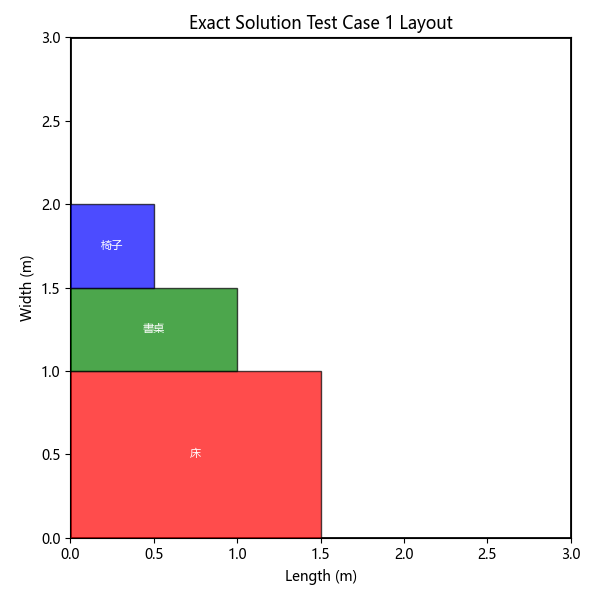
\includegraphics[width=0.8\columnwidth]{exact_layout_test_case_1.png} 
    \caption{CASE1 Optimal Layout using Exact Solver}
    \label{fig:case1_exact_solver}
\end{figure}

\begin{figure}[!htbp]
    \centering
    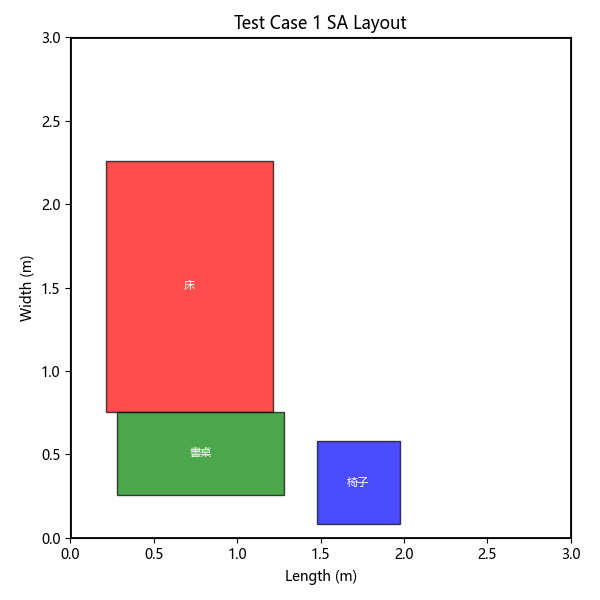
\includegraphics[width=0.8\columnwidth]{sa_layout_test_case_1.png} 
    \caption{CASE1 Optimal Layout using SA}
    \label{fig:case1_sa}
\end{figure}

\FloatBarrier % Ensure CASE1 images are placed

\subsection{CASE2 (5×4m)}
Medium-scale. Exact Solver fails to find a solution (inf), while SA obtains an energy 0 solution in approximately 8.7276 seconds.

\begin{figure}[!htbp]
    \centering
    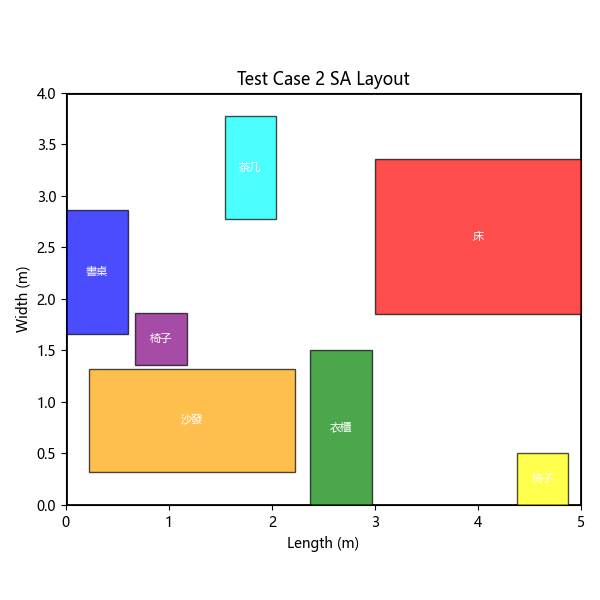
\includegraphics[width=0.8\columnwidth]{sa_layout_test_case_2.png} 
    \caption{CASE2 Optimal Layout using SA}
    \label{fig:case2_sa}
\end{figure}

\FloatBarrier % Ensure CASE2 images are placed

\subsection{CASE3 (2.5×2m)}
Small-scale similar to CASE1. Exact Solver quickly achieves energy 0, and SA can as well but takes longer.

\begin{figure}[!htbp]
    \centering
    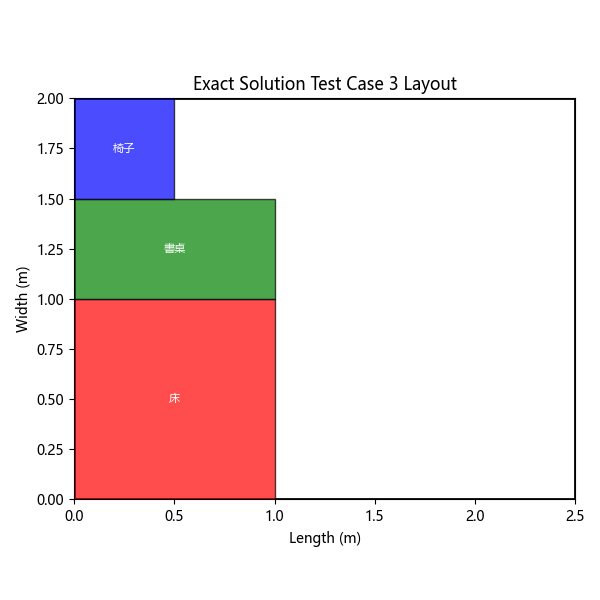
\includegraphics[width=0.8\columnwidth]{exact_layout_test_case_3.png} 
    \caption{CASE3 Optimal Layout using Exact Solver}
    \label{fig:case3_exact_solver}
\end{figure}

\begin{figure}[!htbp]
    \centering
    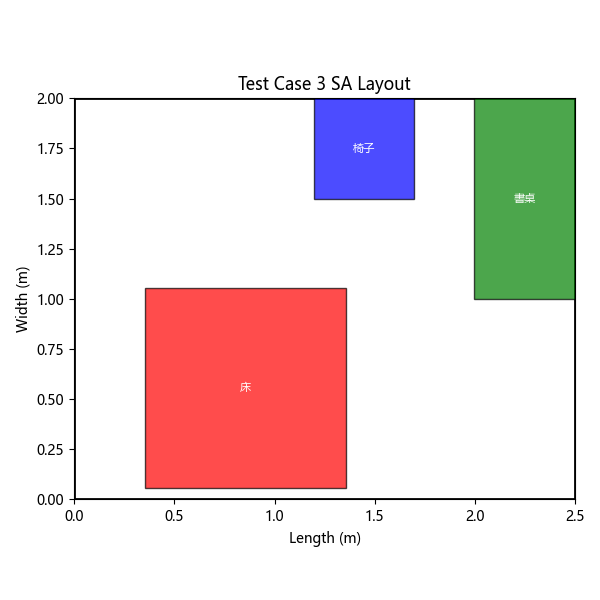
\includegraphics[width=0.8\columnwidth]{sa_layout_test_case_3.png} 
    \caption{CASE3 Optimal Layout using SA}
    \label{fig:case3_sa}
\end{figure}

\FloatBarrier % Ensure CASE3 images are placed

\subsection{CASE4 (6×5m)}
Large-scale. Exact Solver cannot find a solution (N/A), while SA obtains an energy 0.39 solution in approximately 16.3204 seconds.

\begin{figure}[!htbp]
    \centering
    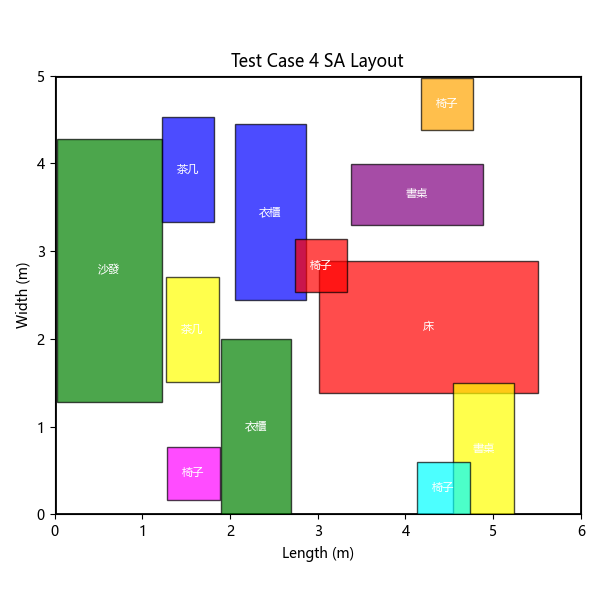
\includegraphics[width=0.8\columnwidth]{sa_layout_test_case_4.png} 
    \caption{CASE4 Optimal Layout using SA}
    \label{fig:case4_sa}
\end{figure}

\FloatBarrier % Ensure CASE4 images are placed

\subsection{Overall Energy Comparison}
The following is the energy comparison graph between SA and Exact Solver:

\begin{figure}[!htbp]
    \centering
    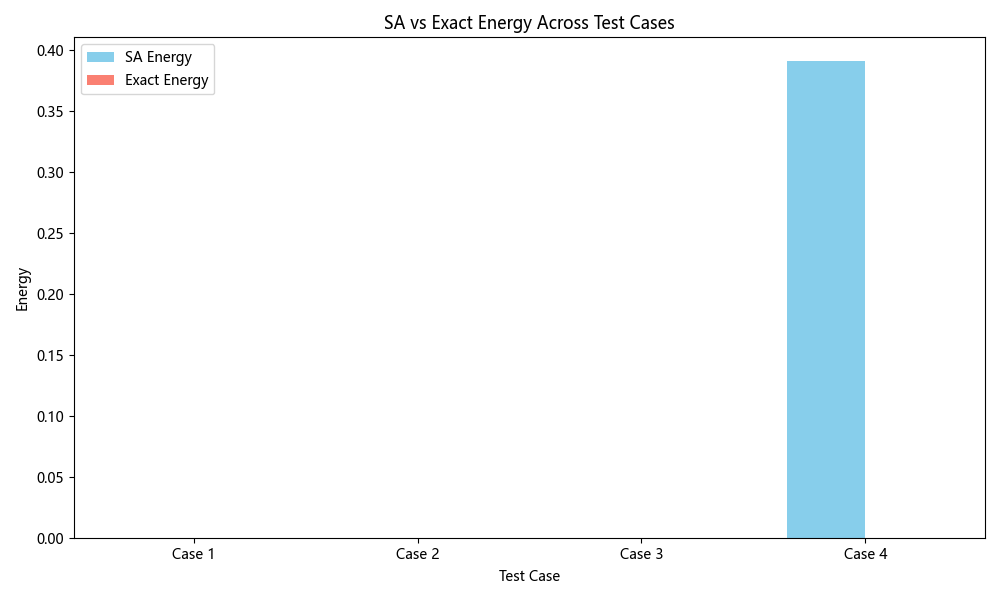
\includegraphics[width=0.8\columnwidth]{energy_comparison.png} 
    \caption{Overall Energy Comparison: Small-scale Exact Solver and SA both achieve 0; Medium to large-scale Exact Solver N/A, SA has feasible solutions}
    \label{fig:energy_comparison}
\end{figure}

\FloatBarrier % Ensure energy comparison graph is placed

\subsection{Overall Time Comparison}
The following is the time comparison graph between SA and Exact Solver:

\begin{figure}[!htbp]
    \centering
    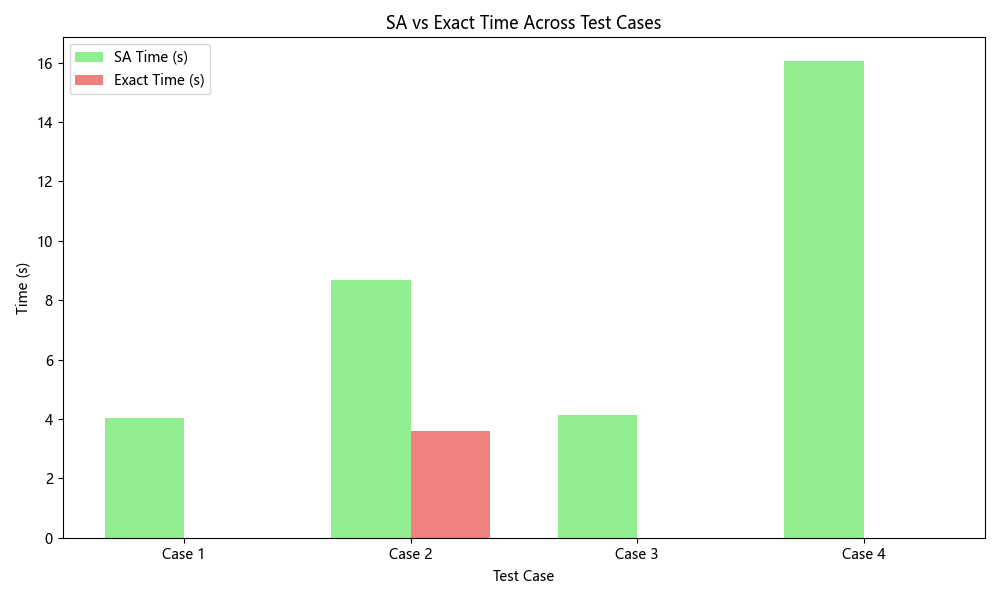
\includegraphics[width=0.8\columnwidth]{time_comparison.png} 
    \caption{Overall Time Comparison: Exact Solver is extremely fast for small problems, SA takes longer; Exact Solver is N/A for medium to large-scale problems, SA takes longer but has solutions}
    \label{fig:time_comparison}
\end{figure}

\FloatBarrier % Ensure time comparison graph is placed

\subsection{Summary of Results in Table}
Table I summarizes the results of the four cases.

\begin{table}[!htbp]
\centering
\caption{Summary of Results for Four Cases}
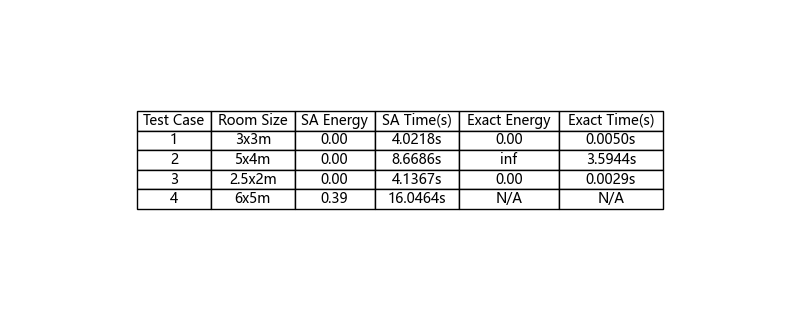
\includegraphics[width=0.8\columnwidth]{results_comparison_table.png} 
\label{tab:results_summary}
\end{table}

\FloatBarrier % Ensure table is placed

\section{Conclusion and Future Work}
This study compares the performance of SA and Exact Solver in room layout optimization problems. The results show:
\begin{itemize}
    \item Small-scale problems: Exact Solver can quickly obtain the optimal solution with energy 0, and SA can also achieve 0 but takes longer.
    \item Medium to large-scale problems: Exact Solver fails to solve (N/A), while SA, although time-consuming, can obtain feasible solutions.
\end{itemize}

Future work may consider hybrid strategies (such as using Exact Solver for local solutions first, then using SA for global optimization) or adding practical constraints to make the results more aligned with real design requirements.

\FloatBarrier % Ensure all floating objects are placed before this point

\begin{thebibliography}{99}
\bibitem{b1} Kirkpatrick, S., Gelatt, C. D., \& Vecchi, M. P. (1983). Optimization by simulated annealing. \textit{Science}, 220(4598), 671–680. \url{https://doi.org/10.1126/science.220.4598.671}

\bibitem{b2} Woeginger, G. J. (2003). Exact algorithms for NP-hard problems: A survey. In Jünger, M., Reinelt, G., \& Rinaldi, G. (Eds.), \textit{Combinatorial Optimization—Eureka, You Shrink! (Lecture Notes in Computer Science, vol. 2570)}. Springer, Berlin, Heidelberg. \url{https://doi.org/10.1007/3-540-36478-1_17}
\end{thebibliography}

\end{document}
